%% implementation

\section{SPHLATCH - An implementation}

This section shows on a quite technical level how a parallel version the Barnes \& Hut tree algorithm has been implemented in C++.

\subsection{Implementing a tree datastructure}
The most common and probably also easiest way to implement a tree datastructure is by using \emph{pointers}. Pointers are a datatype pointing to another datatype, which can be a pointer again. One now defines a node datastructure, which is made up of pointers to others nodes, namely the parent node and the children node. If a child does not exist, corresponding pointer is set to the null pointer. As there may be more than one child, an array is used to store the child pointers with a size corresponding to the maximum number of children. Other information can also be stored in the tree node, for example in the case of a Barnes \& Hut tree the depth and the center coordinates of a cell.
\begin{verbatim}
struct node {
    node* parent;
    node* child[8];    // an octree
    
    // let's save some useful data.
    int depth;
    float centerX, centerY, centerZ;
    ...
}
\end{verbatim}

The tree can now be contructed by letting the nodes point to each other. If we don't want to have to access the tree nodes explicitely, it is necessary to define a \emph{cursor}. The cursor is a node pointer and can therefore point to any node in the tree. Data of the nodes can be accessed through the cursor. 
\begin{verbatim}
...
// assume we have the tree: Root -> Child0 -> Grandchild3
node* Cursor;
Cursor = *Root;               // initialize the Cursor
Cursor = Cursor->child[0];    // Cursor now points to Child0
Cursor->centerX = 42.;        // set centerX of Childo to 42
Cursor = Cursor->child[3];    // Cursor now points to Grandchild3
Cursor = Cursor->parent;      // ... to Child0 again
...
\end{verbatim}

Elementary tree operations can now be implemented, like going up to the parent node or going to a child.\\

Tree walks can be implemented be implemented by recursive functions, so called \emph{recursors}:
\begin{verbatim}
void postorderRecursor() {
    // do something
    useful();
    
    // walk existing children
    for (size_t i = 0; i < 8; i++) {        // assume 8 childs
         if ( Cursor->child[i] != NULL ) {
             goChild(i);
             postorderRecursor();           // recurse
             goParent();
         }
    }
}
...
goRoot();               // go to the root node
postorderRecursor();    // walk the tree
...
\end{verbatim}

The cursor will point to every tree node once in a post order and every time the function \verb|useful()| is executed. A pre-order tree walk or a walk of a subtree can be implemented in a similar fashion.\\

Each time the recursor calls itself, the current context is laid on to the stack, so the stack-depth is incremented by one. On a real-world computer, the stack has a finite size. When we want to walk a tree with mind-blowing depth, the stack depth will increase the deeper we go in the tree and will possibly overflow, leading to a program crash. So is recursion dangerous for tree walks? In the case of Barnes \& Hut trees it is not.\\

This can be shown with a quick back of a napkin calculation: Let's imagine a worst-case scenario with two particles positioned at almost the same coordinates. When trying to insert the second particle at almost the same place like the first particle, the two come to lie in the same cell octant so that a new children cell has to be created at this octant. Each time this happens, the resolution to distinguish the two particles increase by two or in other words, the the difference in coordinates of the particles has to be half as small in order for the tree not to be able to distinguish the two particles again. Or we can also say, one more bit of the binary representation of the particles coordinates have to match each other. Particle coordinates are usually stored as floating point numbers. A floating point number is usually represented according to the \emph{IEEE 754} standard, with 24 bits precision for a single precision float and 53 bits for a double precision float. So in a worst case, the tree gets a depth of around 24 or 53, a depth which can be handled by the stacks of modern computers. And yet this worst-case is very pathological, as a calculation with such high dynamics easily leads to other problems like over- or underflows. Concluding we can say, that recursion for the B\&H-tree walks is not dangerous.

\subsection{Implementing a B\&H-tree}
The gravitational acceleration calculation with a parallelized B\&H-tree like shown before breaks down to 4 major steps: Building the top-tree, inserting the particles and ghosts, calculating the multipole moments and finally calculating the resulting acceleration on the particles. If the tree is not needed any more, the tree has also to be deleted. For this five steps, there exist easy recursive algorithms.

\begin{algorithm}
\caption{}
\begin{algorithmic}
\label{alg:postorder}
\STATE{pick current node}
\FORALL{children}
\STATE{go to child}
\STATE{do post order walk}
\ENDFOR
\end{algorithmic}
\end{algorithm}


recursions

\subsection{Parallizing a particle calculation}

costzone stuff

\subsection{Parallizing a B\&H-tree}

\begin{figure}[htbp]
\begin{center}
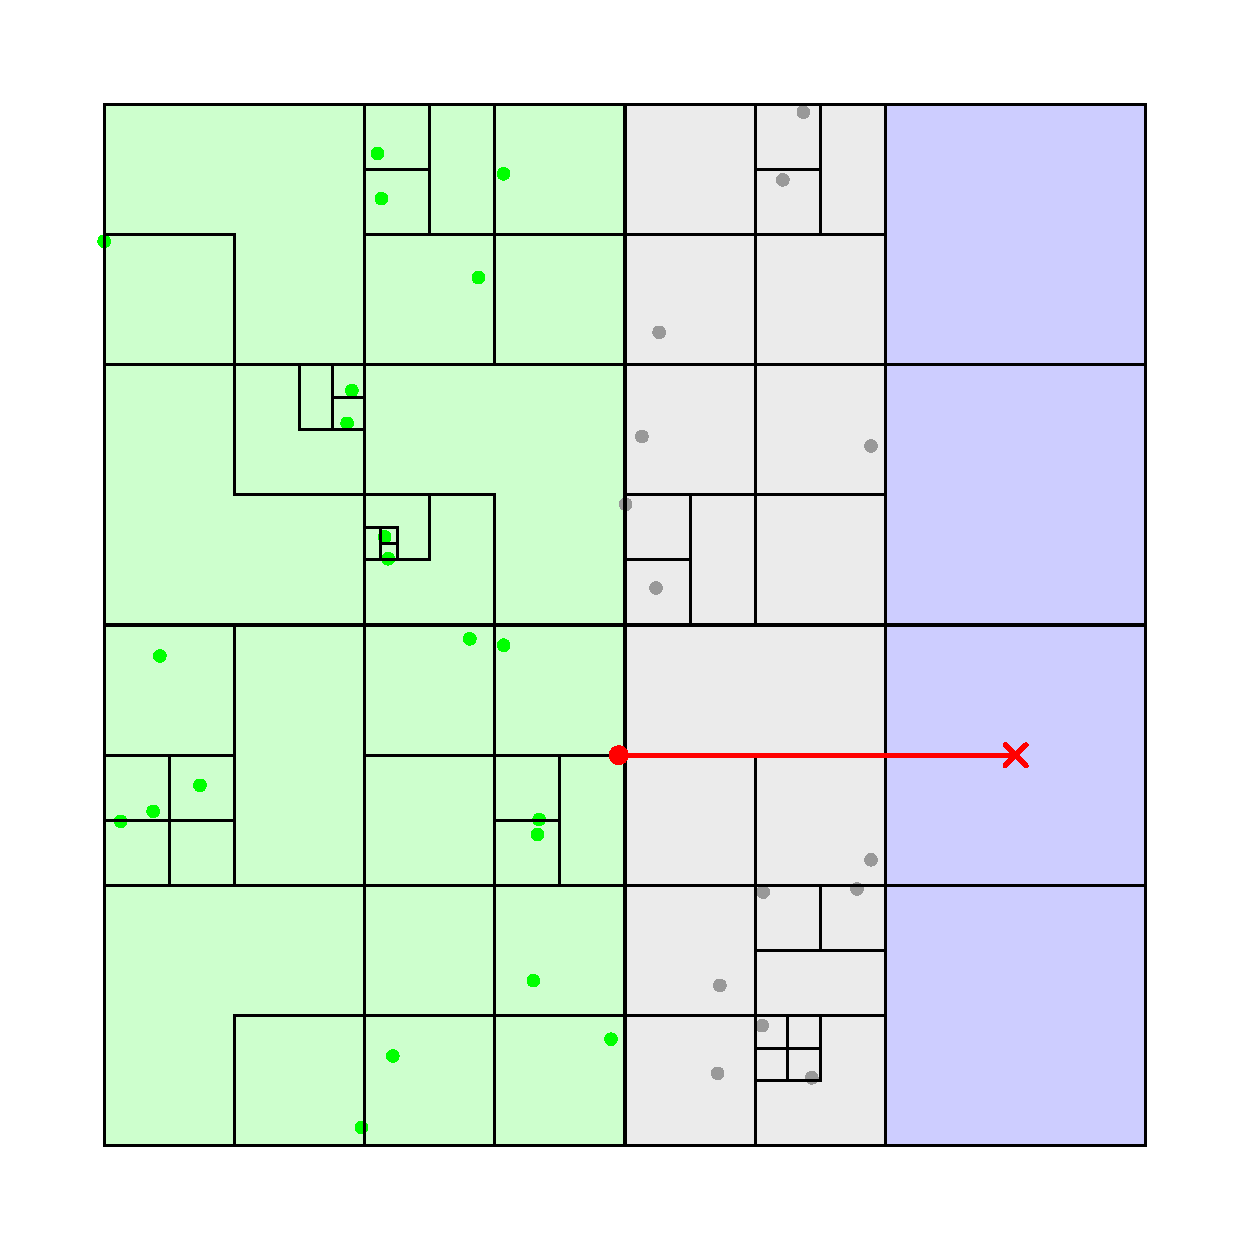
\includegraphics[scale=0.6]{quadtree50_xy_TPL2.pdf}
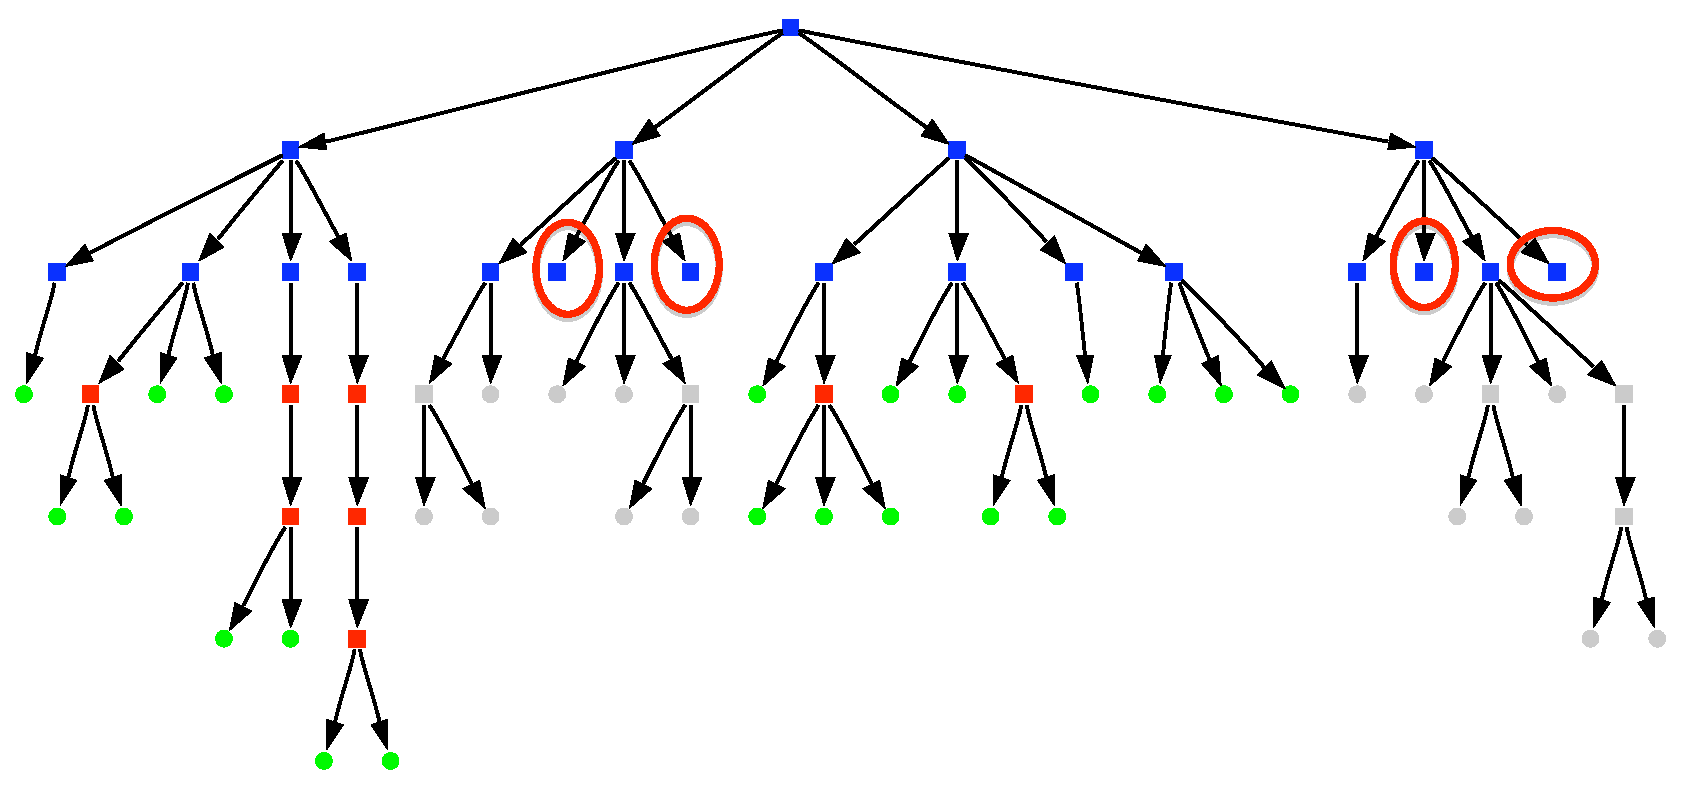
\includegraphics[scale=0.3]{quadtree50_TPL2.pdf}
\caption{the same 50 particles randomly distributed in $2D$}
\caption{A part of the same particle distribution like in figure \ref{fig:2D_BHtree}. The local domain is shaded green and contains 21 particles for which the acceleration has to be calculated. Bordering this zone is the ghost domain shaded grey, for which all particles are known. Beyond that, no particle information is available, only the corresponding parts of the global tree down to top-tree depth are known here. The plot below shows the corresponding tree. Note the filled top-tree nodes without any children nodes, they correspond to the domain where no particle information is available.}
\label{fig:2D_BHtree_costzone}
\end{center}
\end{figure}

node specialization: toptree node, local vs. non-local nodes and particles
toptree recursion
costzone vs. toptree business
advantage: bulk communication
disadvantage: high memory usage